% !TEX program = xelatex
\documentclass[11pt, letterpaper]{article}

\usepackage[margin=1in]{geometry}

%  FONTS (XeLaTeX)
\usepackage{fontspec}
\setmainfont{Poppins}
\newfontfamily\displayfont{Poppins}[BoldFont={Poppins Bold}]
\newfontfamily\lightfont{Poppins Light}

\makeatletter
\renewcommand{\textsc}[1]{%
  \begingroup
  \addfontfeature{LetterSpace=4}%
  {\fontsize{\f@size}{\f@baselineskip}\selectfont\MakeUppercase{#1}}%
  \endgroup
}
\makeatother

\usepackage{array}
\usepackage{longtable}
\usepackage{tabularx}
\usepackage{xcolor}
\usepackage{colortbl}
\usepackage[hidelinks]{hyperref}
\usepackage{pifont}


\usepackage{fancyhdr}
\usepackage{titlesec}
\usepackage{parskip}

\usepackage{amsmath, amssymb}
\usepackage{microtype}
\emergencystretch=3em
\usepackage{lastpage}

\usepackage{booktabs}
\usepackage{enumitem}
\usepackage{tikz}
\usetikzlibrary{calc,shapes.geometric,decorations.pathmorphing}
\usepackage{graphicx}
\usepackage{url}
\usepackage{float}
\usepackage{pdflscape}
\usepackage{multirow}
\usepackage{makecell}
\usepackage{subcaption}

\usepackage{listings}
\usepackage[most, breakable]{tcolorbox}
\usepackage{capt-of}

%  COLOR PALETTE
\definecolor{charcoal}{RGB}{26,24,23}
\definecolor{charcoal2}{RGB}{40,37,35}
\definecolor{terracotta}{RGB}{196,93,58}
\definecolor{terracottadark}{RGB}{150,66,38}
\definecolor{gold}{RGB}{206,164,89}
\definecolor{cream}{RGB}{250,246,239}
\definecolor{darkgray}{RGB}{68,63,60}
\definecolor{midgray}{RGB}{120,113,108}
\definecolor{medgray}{RGB}{163,155,148}
\definecolor{lightgray}{RGB}{230,225,218}
\definecolor{palegray}{RGB}{248,245,240}
\definecolor{rulecolor}{RGB}{210,201,192}
\definecolor{codegray}{RGB}{247,244,239}
\definecolor{sagegreen}{RGB}{122,140,110}

\newcolumntype{Y}{>{\raggedright\arraybackslash}X}
\newcolumntype{L}[1]{>{\raggedright\arraybackslash}p{#1}}
\newcolumntype{C}[1]{>{\centering\arraybackslash}p{#1}}
\newcolumntype{R}[1]{>{\raggedleft\arraybackslash}p{#1}}
\renewcommand{\arraystretch}{1.3}
\setlength{\tabcolsep}{6pt}

\lstset{
  basicstyle=\ttfamily\small,
  breaklines=true,
  frame=single,
  backgroundcolor=\color{codegray},
  rulecolor=\color{rulecolor},
  keywordstyle=\bfseries\color{terracottadark},
  stringstyle=\color{midgray},
  commentstyle=\itshape\color{medgray},
  showstringspaces=false,
  tabsize=2,
  captionpos=b,
  numbers=left,
  numberstyle=\tiny\color{medgray},
  numbersep=8pt,
  xleftmargin=15pt,
  framexleftmargin=15pt
}

\tcbset{
  notebox/.style={
    colback=palegray, colframe=terracotta, left=8pt, right=8pt,
    fonttitle=\bfseries\small, coltitle=white,
    attach boxed title to top left={yshift=-2mm, xshift=4mm},
    boxed title style={colback=terracotta, colframe=terracotta, sharp corners},
    breakable, enhanced, sharp corners=downhill
  },
  warningbox/.style={
    colback=palegray, colframe=charcoal2, left=8pt, right=8pt,
    fonttitle=\bfseries\small, coltitle=white,
    attach boxed title to top left={yshift=-2mm, xshift=4mm},
    boxed title style={colback=charcoal2, colframe=charcoal2, sharp corners},
    breakable, enhanced
  },
  placeholderbox/.style={
    colback=cream, colframe=gold, left=8pt, right=8pt, boxrule=1.1pt,
    fonttitle=\bfseries\small, coltitle=terracottadark, breakable, enhanced
  },
  shotbox/.style={
    colback=palegray, colframe=medgray, left=6pt, right=6pt, top=6pt, bottom=6pt,
    boxrule=0.6pt, unbreakable, enhanced
  }
}

\newcommand{\ticon}[1]{%
  \tikz[baseline=-0.55ex]{\node[circle, draw=white, line width=0.7pt, text=white,
    font=\bfseries\fontsize{6.5}{6.5}\selectfont, inner sep=0pt, minimum size=1.25em] {#1};}%
}

\newcommand{\stepbadgeraw}[1]{%
  \tikz[baseline=(n.base)]{\node[circle, fill=terracotta, text=cream,
    font=\bfseries\small, inner sep=0pt, minimum size=1.55em] (n) {#1};}%
}
\makeatletter
\@for\stepbadgen:=1,2,3,4,5,6,7,8,9,10,11,12,13,14,15,16,17,18,19,20,21,22,23,24,25,26,27,28,29,30\do{%
  \expandafter\newsavebox\csname stepbadgebox\stepbadgen\endcsname
  \expandafter\sbox\csname stepbadgebox\stepbadgen\endcsname{\stepbadgeraw{\stepbadgen}}%
}
\makeatother
\usepackage{etoolbox}
\newrobustcmd{\stepbadge}[1]{\usebox{\csname stepbadgebox#1\endcsname}}

\newcommand{\accentsq}{\raisebox{0.14em}{\tikz{\fill[gold] (0,0) rectangle (0.32em,0.32em);}}}

\newcommand{\secref}[1]{\hyperref[#1]{\textcolor{terracottadark}{\bfseries Section~\ref*{#1}}}}

\newcommand{\sectionbadge}[1]{%
  \tikz[baseline=(s.base)]{\node[fill=terracotta, text=cream, rounded corners=3pt,
    font=\displayfont\bfseries\Large, inner sep=7pt, minimum width=1.5em,
    minimum height=1.35em, align=center] (s) {#1};}%
}

\newcommand{\screenshot}[3][0.75\linewidth]{%
  \begingroup\centering
  \IfFileExists{#2}{%
    \includegraphics[width=#1]{#2}\par
    \captionof{figure}{#3}\par
  }{%
    \begin{tcolorbox}[shotbox, width=#1]
      \centering
      \vspace{2pt}
      {\small\textbf{\textcolor{terracottadark}{Screenshot placeholder}}}\\[4pt]
      {\footnotesize\ttfamily\textcolor{midgray}{\detokenize{#2}}}
      \vspace{2pt}
    \end{tcolorbox}
    \captionof{figure}{#3}\par
  }%
  \endgroup
}

\newcommand{\stepshot}[4][0.75\linewidth]{%
  \begin{minipage}[t]{0.94\linewidth}
    #2\par\vspace{6pt}
    \screenshot[#1]{#3}{#4}
  \end{minipage}%
}

\newcommand{\paragraphshot}[4][0.75\linewidth]{%
  \begin{minipage}{\linewidth}
    #2\par\vspace{6pt}
    \screenshot[#1]{#3}{#4}
  \end{minipage}\par\vspace{4pt}
}

\newlist{steplist}{enumerate}{1}
\setlist[steplist]{label=\stepbadge{\thesteplisti}, leftmargin=2.3em, itemsep=10pt,
  topsep=6pt, parsep=2pt, align=left}

\renewcommand{\labelitemi}{\textcolor{terracotta}{\small\textbullet}}

\pagestyle{fancy}
\fancyhf{}
\fancyhead[L]{\small\textcolor{midgray}{\textsc{Bland2Grand}}\ \textcolor{rulecolor}{|}\ \textcolor{midgray}{Maker's Guide}}
\fancyhead[R]{\small\textcolor{terracottadark}{\textbf{v1.0}}}
\fancyfoot[L]{\small\textcolor{medgray}{VEJ}}
\fancyfoot[R]{\small\textcolor{medgray}{Page \thepage\ of \pageref{LastPage}}}

\renewcommand{\headrulewidth}{0.8pt}
\renewcommand{\footrulewidth}{0.6pt}
\renewcommand{\headrule}{\color{terracotta}\hrule width\headwidth height\headrulewidth}
\renewcommand{\footrule}{\color{rulecolor}\hrule width\headwidth height\footrulewidth}
\setlength{\headheight}{15pt}

\titleformat{\section}
  {\normalfont}
  {\sectionbadge{\thesection}}
  {0.6em}
  {\displayfont\bfseries\fontsize{22}{26}\selectfont\color{charcoal}}
  [\vspace{4pt}{\color{terracotta}\titlerule[1.3pt]}\vspace{10pt}]

\titleformat{\subsection}
  {\displayfont\bfseries\fontsize{14}{17}\selectfont\color{terracottadark}}
  {\textcolor{gold}{\thesubsection}}{0.6em}{}

\titleformat{\subsubsection}
  {\displayfont\bfseries\fontsize{11}{13}\selectfont\color{darkgray}}
  {\accentsq}{0.5em}{}

\titlespacing*{\section}{0pt}{22pt}{12pt}
\titlespacing*{\subsection}{0pt}{16pt}{6pt}
\titlespacing*{\subsubsection}{0pt}{12pt}{5pt}

\usepackage{tocloft}
\renewcommand{\cftsecfont}{\displayfont\bfseries\color{charcoal}}
\renewcommand{\cftsecpagefont}{\color{terracottadark}}
\renewcommand{\cftsubsecfont}{\color{darkgray}}
\renewcommand{\cftsubsecpagefont}{\color{midgray}}
\renewcommand{\cftsecleader}{\color{rulecolor}\cftdotfill{\cftdotsep}}
\renewcommand{\cftsubsecleader}{\color{rulecolor}\cftdotfill{\cftdotsep}}
\setlength{\cftbeforesecskip}{10pt}

\begin{document}

\begin{titlepage}
\pagecolor{charcoal}\color{cream}
\thispagestyle{empty}
\begin{tikzpicture}[remember picture, overlay]
  % top / bottom bands 
  \fill[terracotta] (current page.north west) rectangle ([yshift=-3.6cm]current page.north east);
  \fill[charcoal] ([yshift=-3.6cm]current page.north west) -- ([yshift=-4.6cm]current page.north west) --
                  ([xshift=6cm,yshift=-3.6cm]current page.north west) -- cycle;
  \fill[gold] (current page.south west) rectangle ([yshift=2.4cm]current page.south east);
  \fill[charcoal] ([yshift=2.4cm]current page.south east) -- ([yshift=3.2cm]current page.south east) --
                  ([xshift=-6cm,yshift=2.4cm]current page.south east) -- cycle;

  % corner registration marks (blueprint / spec-sheet feel) top corners, just below the terracotta band
  \draw[gold, line width=0.8pt]
    ([xshift=1.1cm, yshift=-4.9cm]current page.north west) -- ++(0.55cm,0)
    ([xshift=1.1cm, yshift=-4.9cm]current page.north west) -- ++(0,-0.55cm);
  \draw[gold, line width=0.8pt]
    ([xshift=-1.1cm, yshift=-4.9cm]current page.north east) -- ++(-0.55cm,0)
    ([xshift=-1.1cm, yshift=-4.9cm]current page.north east) -- ++(0,-0.55cm);

  % bottom corners, just above the gold band
  \draw[gold, line width=0.8pt]
    ([xshift=1.1cm, yshift=3.2cm]current page.south west) -- ++(0.55cm,0)
    ([xshift=1.1cm, yshift=3.2cm]current page.south west) -- ++(0,0.55cm);
  \draw[gold, line width=0.8pt]
    ([xshift=-1.1cm, yshift=3.2cm]current page.south east) -- ++(-0.55cm,0)
    ([xshift=-1.1cm, yshift=3.2cm]current page.south east) -- ++(0,0.55cm);
\end{tikzpicture}

\vspace*{\fill}
\vspace{0.7cm} % compensates for the top band being taller than the bottom band

\begin{center}

  % eyebrow badge 
  \tikz{\node[draw=terracotta, line width=0.8pt, rounded corners=1pt,
    text=terracotta, font=\bfseries\fontsize{7}{7}\selectfont,
    inner xsep=10pt, inner ysep=5pt] {\addfontfeature{LetterSpace=18}TECHNICAL MANUAL};}

  \vspace{0.9cm}

  {\fontsize{10}{12}\selectfont\textcolor{cream}{\addfontfeature{LetterSpace=22}BLAND2GRAND}}

  \vspace{1.6cm}

  
\includegraphics[width=5.2cm]{images/logo.png}

  \vspace{1.6cm}

  \textcolor{terracotta}{\rule{0.16\textwidth}{1.2pt}}\ \raisebox{-0.09em}{\textcolor{gold}{\footnotesize\ding{72}}}\ \textcolor{terracotta}{\rule{0.16\textwidth}{1.2pt}}

  \vspace{0.5cm}

  {\fontsize{29}{33}\selectfont\color{gold}\bfseries Maker's Guide}\\[0.5cm]
  {\fontsize{12.5}{16}\selectfont\color{lightgray}\itshape
   The Smart, Autonomous Carousel\\ Spice Dispenser}

  \vspace{1.6cm}

  \textcolor{rulecolor!40}{\rule{0.7\textwidth}{0.5pt}}\\[0.4cm]
  {\footnotesize\color{cream}
   \addfontfeature{LetterSpace=8}\textbf{VERSION 1.0}
   \hspace{0.6cm}\textcolor{terracotta}{|}\hspace{0.6cm}
   \addfontfeature{LetterSpace=8}REV.\ \today
   \hspace{0.6cm}\textcolor{terracotta}{|}\hspace{0.6cm}
   \addfontfeature{LetterSpace=8}DOC.\ B2G-MG-001}

\end{center}

\vspace*{\fill}
\vspace{0.7cm}

\end{titlepage}

\pagecolor{white}\color{black}
\newpage
{\hypersetup{linkcolor=terracottadark}\tableofcontents}
\newpage

\section{Introduction}

This System Manual is written for someone who has the printed/purchased parts to build one in front of them and wants to assemble it and get it running. It covers two supported controller boards:

\textbf{\textcolor{terracottadark}{Arduino UNO Q}}\\
The primary, currently supported build. The Flask backend,
dispense logic, and MCU sketch all run on a single board,
launched through Arduino App Lab. Start here.

\vspace{0.5em}

\textbf{\textcolor{terracottadark}{Arduino UNO R4 WiFi}}\\
The original build. The backend and frontend run on a
separate laptop, communicating with the Arduino over a
mobile hotspot.

Follow \secref{sec:assembly} to physically assemble the machine, then \secref{sec:code-setup} to install and launch the software for whichever board you have.

\begin{tcolorbox}[notebox, title={\ticon{i}\ \ At a Glance}]

\arrayrulecolor{gold}

\noindent
\begin{tabular}{c!{\color{gold}\vrule width 1pt}c!{\color{gold}\vrule width 1pt}c}

\hspace*{-0.35cm}
\parbox{0.28\linewidth}{\centering
\textbf{\small\textcolor{terracottadark}{Build Time}}\\[6pt]
\footnotesize A weekend for assembly, an afternoon for software
}
&
\parbox{0.28\linewidth}{\centering
\textbf{\small\textcolor{terracottadark}{Skill Level}}\\[6pt]
\footnotesize Intermediate --- soldering, 3D printing, basic CLI
}
&
\hspace*{0.75cm}
\parbox{0.28\linewidth}{\centering
\textbf{\small\textcolor{terracottadark}{Boards Supported}}\\[6pt]
\footnotesize UNO Q (recommended), UNO R4 WiFi
}

\end{tabular}

\end{tcolorbox}

\section{Assembly}
\label{sec:assembly}

\begin{tcolorbox}[placeholderbox, title={Section In Progress}]
\small
This section will walk through the full mechanical and electrical assembly of Bland2Grand: printing and preparing parts, assembling the carousel and cycloidal gearbox, mounting the auger modules, wiring the motors, drivers, load cell, and controller board, and closing up the enclosure. Content to be added.
\end{tcolorbox}

\subsection{Parts and Tools Needed}
\textit{Placeholder --- bill of materials and tools list.}

\subsection{Printing the Parts}
\textit{Placeholder --- print settings, orientation, and material notes.}

\subsection{Mechanical Assembly}
\textit{Placeholder --- carousel, gearbox, auger modules, tower frame.}

\subsection{Electrical Wiring}
\textit{Placeholder --- motors, drivers, load cell, controller board wiring diagram.}

\subsection{Final Checks Before Power-On}
\textit{Placeholder --- pre-power checklist.}

\section{Code and Software Setup}
\label{sec:code-setup}

All source code for Bland2Grand is hosted on GitHub: \href{https://github.com/ElliottStarosta/Bland2Grand}{\textcolor{terracottadark}{\url{github.com/ElliottStarosta/Bland2Grand}}}. The repository contains separate, self-contained builds for each supported board. Set up the one that matches your hardware.

\subsection{Arduino UNO Q Setup (Recommended)}
\label{sec:unoq-setup}

The UNO Q build runs the whole system (MCU sketch, Flask backend, REST API, SSE stream, and the built React frontend) as a single App Lab app on the board itself. There is no separate laptop backend/frontend to run.

\subsubsection{Phase 1: Download the Project}

\begin{steplist}
  \item \stepshot{Navigate to the \href{https://github.com/ElliottStarosta/Bland2Grand}{Bland2Grand GitHub repository}.}{images/uq_github_repo.png}{The Bland2Grand GitHub repository page.}

  \item \stepshot{Locate and click on the latest release.}{images/uq_latest_release.png}{Latest release on the Releases page.}

  \item \stepshot{Scroll to the \textbf{Assets} section at the bottom of the release.}{images/uq_assets_section.png}{Assets section at the bottom of a release.}

  \item \stepshot{Download the zip file: \texttt{Bland2Grand\_Arduino\_Uno\_Q.zip}.}{images/uq_zip_download.png}{Downloading \texttt{Bland2Grand\_Arduino\_Uno\_Q.zip} from the Assets list.}

\end{steplist}

\subsubsection{Phase 2: Deploy to Arduino / App Lab}

\begin{steplist}[start=5]
  \item Open \textbf{App Lab}.
  \item \stepshot{Select your board.}{images/uq_applab_board_select.png}{Selecting the connected UNO Q board in App Lab.}

  \item \stepshot{Click \textbf{Create new app} in the top right-hand corner.}{images/uq_applab_create_app.png}{The ``Create new app'' button in App Lab.}

  \item Click \textbf{Import App} and select the \texttt{.zip} file you downloaded in Phase 1.
\end{steplist}

\subsubsection{Phase 3: Configure API Credentials}

The AI-assisted custom blend feature calls out to OpenRouter. An API key is required for this feature to work (the rest of the app --- search, dispensing, calibration --- works without it).

\begin{steplist}[start=9]
  \item Go to the \href{https://openrouter.ai/sign-in?redirect_url=https\%3A\%2F\%2Fopenrouter.ai\%2Fworkspaces\%2Fdefault\%2Fkeys}{OpenRouter keys page}.
  \item \stepshot{Click \textbf{New Key}.}{images/uq_openrouter_newkey.png}{The ``New Key'' button on the OpenRouter keys page.}

  \item \stepshot{Fill out the required information.}{images/uq_openrouter_keyform.png}{OpenRouter new key creation form.}

  \item \stepshot{Copy the key shown on the confirmation screen right away --- OpenRouter will not show it to you again.}{images/uq_new_key_reveal.png}{The one-time key reveal screen after creating a key.}

  \item \stepshot{Update the relevant environment variables for the app, most importantly \texttt{OPENROUTER\_API\_KEY}.}{images/uq_env_config.png}{Example environment configuration for the UNO Q app.}
\end{steplist}

\begin{tcolorbox}[warningbox, title={\ticon{!}\ \ Keep your API key private}]
\small
Treat your OpenRouter key like a password: don't commit it to a public repository, share it in screenshots, or paste it into chat tools. If a key is ever exposed, revoke it from the OpenRouter dashboard and generate a new one.
\end{tcolorbox}

\subsubsection{Phase 4: Run the Application}

\begin{steplist}[start=13]
  \item \stepshot{Set the application to run on startup by clicking the down arrow at the top left-hand side of the screen, next to ``Bland2Grand''.}{images/uq_startup_dropdown.png}{The startup dropdown next to the app name in App Lab.}

  \item \stepshot{Toggle the \textbf{Run at startup} option to enabled.}{images/uq_run_at_startup_toggle.png}{Enabling the ``Run at startup'' toggle.}

  \item Click the \textbf{Run} button in the top right-hand corner of the screen. App Lab uploads the MCU sketch and starts the Flask app on the board's Linux side.
  \item Access the web server by opening the board's address on port \textbf{5000} (the port declared in \texttt{app.yaml}) in your browser.
  \item You are now ready to use Bland2Grand.
\end{steplist}

\begin{tcolorbox}[notebox, title={\ticon{i}\ \ Why enable Run at startup}]
\small
With \textbf{Run at startup} enabled, the UNO Q automatically relaunches the Bland2Grand app any time it's powered on or rebooted, so you don't need App Lab open to bring the machine back up after a power cycle.
\end{tcolorbox}

\begin{tcolorbox}[notebox, title={\ticon{i}\ \ No separate frontend server}]
\small
Unlike the UNO R4 build below, the UNO Q serves the built React frontend directly from the same Flask app that handles the API, so there is nothing else to start or forward --- one board, one port, one app.
\end{tcolorbox}

\subsection{Arduino UNO R4 WiFi Setup}
\label{sec:unor4-setup}

The UNO R4 build splits the system across three pieces: firmware on the Arduino, a Flask backend, and a React frontend, both of the latter run on a laptop and communicate with the Arduino over WiFi. This section assumes the hardware is already assembled and wired per \secref{sec:assembly}, and that the \texttt{Bland2Grand\_Arduino}, \texttt{bland2grand-backend}, and \texttt{bland2grand-frontend} folders (and the provided \texttt{.vscode/tasks.json}) are on the laptop that will run the software.

\subsubsection{Hardware Power-On}

\begin{steplist}
  \item Place the machine on a flat, level surface --- the load cell platform must stay level to within 2$^\circ$ for accurate readings.
  \item Connect the 24\,V power supply to the wall.
  \item Confirm each of the 8 spice containers is loaded and seated.
  \item Place an empty bowl on the scale platform. The scale tares before each dispense, so the exact bowl weight does not matter.
  \item Make sure the host laptop is powered on and ready to start its mobile hotspot (see below) --- the Arduino and the phone running the web app both need to join it.
\end{steplist}

\subsubsection{Launching the Software}

\paragraphshot{All software is launched from VS Code using the provided \texttt{tasks.json}. Open the project workspace in VS Code, then open the Command Palette with \textbf{Ctrl+Shift+P} and select \textbf{Tasks: Run Task}.}{images/r4_tasks_run.png}{VS Code Command Palette showing ``Tasks: Run Task'' selected.}

Two compound tasks are available:

\begin{center}
\begin{tabular}{|L{5cm}|L{8.5cm}|}
\hline
\rowcolor{terracotta}
\textcolor{white}{\textbf{Task Name}} & \textcolor{white}{\textbf{What it does}} \\\hline
\textbf{Bland2Grand: Full Stack} & Flashes firmware to the Arduino, opens the serial monitor, starts the Flask backend, and starts the Vite frontend --- all in parallel. Use this for a full bring-up from scratch. \\\hline
\rowcolor{lightgray}
\textbf{Bland2Grand: Backend + Frontend} & Starts only the Flask backend and the Vite frontend. Use this when the Arduino is already flashed and running. This is the task to run for a demo. \\\hline
\end{tabular}
\end{center}

\paragraphshot{\begin{tcolorbox}[notebox, unbreakable, title={\ticon{i}\ \ What \textbf{Full Stack} does automatically}]
\small
The \textbf{Arduino: Flash + Serial} subtask does three things before flashing: it starts the Windows mobile hotspot (so the Arduino has a network to connect to), kills any open serial monitor that would block the port, then runs \texttt{pio run --target upload} followed by \texttt{pio device monitor --baud 9600}. No manual hotspot setup or port management is needed.
\end{tcolorbox}}{images/r4_task_picker.png}{VS Code task picker showing the available Bland2Grand tasks.}

Once the \textbf{Backend + Frontend} task is running, the web app is accessible from any device on the same network at:

\begin{center}
\colorbox{palegray}{\texttt{\textcolor{terracottadark}{http://\{laptop\_ip\}:5173}}}
\end{center}

The laptop's IP address is printed in the Vite terminal panel when it starts. On the Arduino's serial monitor you will also see the IP it received from the hotspot, which confirms the two devices are on the same subnet.
\subsubsection{First-Time Backend Setup}

If this is the first time running the backend on this laptop, set it up once before using the VS Code tasks:

\begin{lstlisting}[language=bash]
cd bland2grand-backend
python -m venv venv
venv\Scripts\activate
pip install -r requirements.txt
python seed_recipes.py
\end{lstlisting}

\newpage
Create a \texttt{.env} file in \texttt{bland2grand-backend/}:

\begin{lstlisting}
ARDUINO_URL=http://192.168.x.x
OPENROUTER_API_KEY=YOUR_KEY_HERE
AI_MODEL=anthropic/claude-3-haiku
DATABASE_PATH=bland2grand.db
FLASK_PORT=5000
MOCK_ARDUINO=true
\end{lstlisting}

\begin{lstlisting}[language=bash]
cd bland2grand-frontend
npm install
\end{lstlisting}

Open \texttt{Bland2Grand\_Arduino} in PlatformIO once to confirm it builds before relying on the VS Code task to flash it.

\begin{tcolorbox}[warningbox, title={\ticon{!}\ \ Set \texttt{MOCK\_ARDUINO=false} for a real run}]
\small
\texttt{MOCK\_ARDUINO=true} simulates dispensing in software with no hardware attached --- useful for testing the app without the machine. Set it to \texttt{false} once the Arduino is flashed and wired, so the backend talks to the real hardware.
\end{tcolorbox}

\section{Using Bland2Grand}
\label{sec:using}

Once your board is flashed and the app is running (\secref{sec:unoq-setup} or \secref{sec:unor4-setup}), everything from here on is identical regardless of which board you built. You interact with Bland2Grand entirely through a web app on your phone: the machine handles all indexing, dispensing, and weight confirmation autonomously and reports the result back in real time.

\begin{center}
  \IfFileExists{images/user_guide/system_front_view.jpeg}{%
    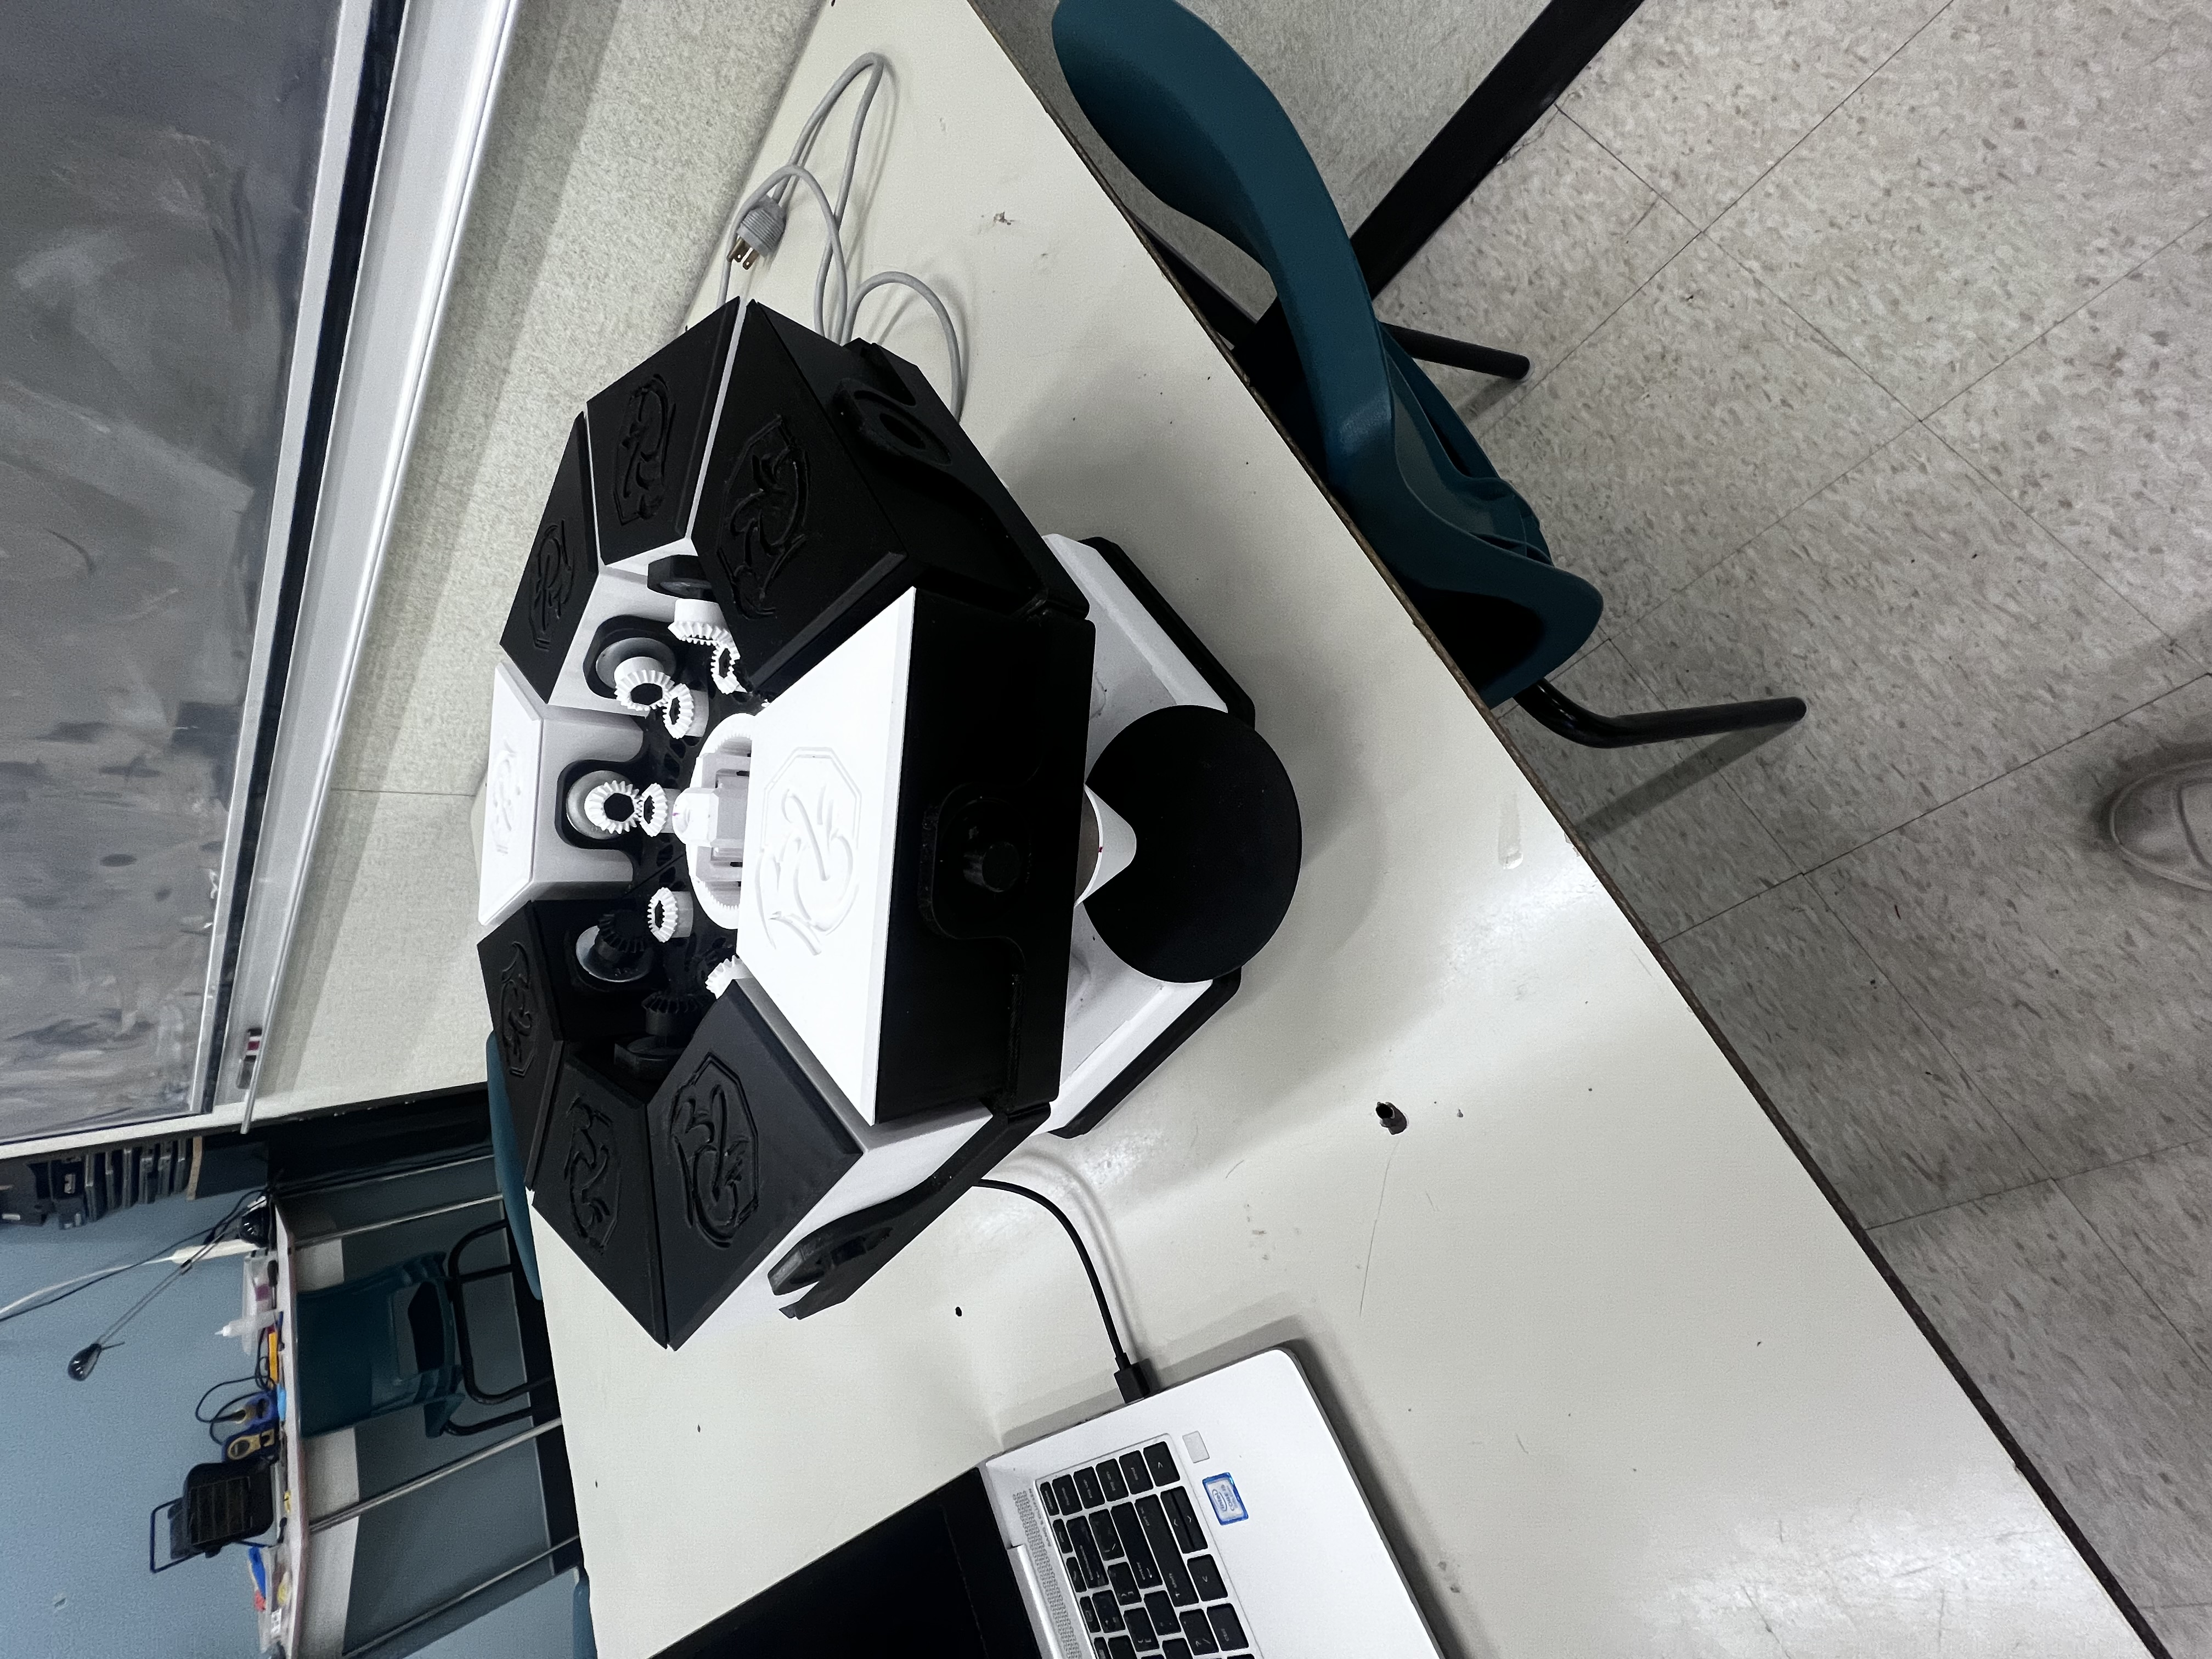
\includegraphics[width=0.45\linewidth,angle=-90]{images/user_guide/system_front_view.jpeg}\par
    \captionof{figure}{Bland2Grand assembled system, ready to dispense.}\par
  }{%
    \begin{tcolorbox}[shotbox, width=0.45\linewidth]
      \centering
      \vspace{2pt}
      {\small\textbf{\textcolor{terracottadark}{Screenshot placeholder}}}\\[4pt]
      {\footnotesize\ttfamily\textcolor{midgray}{\detokenize{images/user_guide/system_front_view.jpeg}}}
      \vspace{2pt}
    \end{tcolorbox}
    \captionof{figure}{Bland2Grand assembled system, ready to dispense.}\par
  }
\end{center}

\subsection{Powering On and Preparing to Dispense}

\begin{steplist}
  \item \textbf{Place the machine on a flat, level surface.} The load cell platform must stay level to within 2\textdegree\ for accurate readings --- avoid uneven countertops or surfaces that vibrate.

  \item \textbf{Connect power to the board.} 24\,V for the UNO R4 build, or the UNO Q's own power input if that's your build.

  \item \textbf{Verify spice containers are loaded.} Each of the 8 slots should hold its designated spice (see the slot map in \secref{sec:refill}). Friction-fit lids pull straight off --- do not twist.

  \item \stepshot{\textbf{Place an empty bowl on the scale platform.} Sit it flat and centred --- the scale tares before each dispense, so the exact bowl weight doesn't matter.}{images/user_guide/bowl_onscale.jpg}{Bowl placed on the scale platform at the base of the machine.}

  \item \textbf{Confirm the app is reachable.} Open the board's URL on your phone (port \textbf{5000} for UNO Q, or \texttt{http://\{laptop\_ip\}:5173} for UNO R4) and make sure the phone is on the same network as the board.
\end{steplist}

\begin{tcolorbox}[notebox, title={\ticon{i}\ \ Same app, either board}]
\small
The interface below is served identically whether the Flask app is running on the UNO Q itself or on a laptop for the UNO R4 build. Once the URL loads, the rest of this section applies exactly as written.
\end{tcolorbox}

\subsection{Using the Mobile Web App}

\subsubsection{Idle Screen: Tap to Wake}

When you first open the URL, the idle screen appears: ambient coloured orbs drift across a dark background with the Bland2Grand logo and a pulsing tap indicator. Tap anywhere to wake the app.

\begin{center}
\screenshot[0.3\linewidth]{images/user_guide/idle_screen.png}{Idle screen. Tap anywhere to continue.}
\end{center}

\newpage
\subsubsection{Search Screen: Find a Recipe}

The search screen offers three ways to find a recipe:

\begin{enumerate}[leftmargin=1.5em, itemsep=4pt]
  \item \textbf{Type a dish name} into the search bar. Results appear automatically after a 2.5-second pause. If no local match exists, the AI generates a blend and saves it to the database for next time.
  \item \textbf{Tap a Featured Blend} tile to jump directly to a popular recipe without searching.
  \item \textbf{Tap a cuisine category} (Mexican, Indian, Italian, etc.) to browse everything in that category.
\end{enumerate}

\begin{center}
\screenshot[0.4\linewidth]{images/user_guide/search_screen.png}{Search screen showing the search bar, featured blends, and cuisine category grid.}
\end{center}

If the dish isn't in the local database yet, an AI loading overlay appears while the blend is generated --- this takes 1--3 seconds and only happens once per unique dish name; every future search for the same dish is served instantly from the cache.

\begin{figure}[H]
  \centering
  \begin{minipage}{0.45\linewidth}
    \centering
    
\includegraphics[width=\linewidth]{images/user_guide/ai_loading.png}
    \small\textit{AI generating a blend}
  \end{minipage}
  \hfill
  \begin{minipage}{0.45\linewidth}
    \centering
    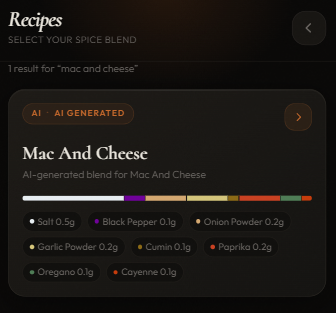
\includegraphics[width=\linewidth]{images/user_guide/ai_result.png}
    \small\textit{Generated result}
  \end{minipage}
  \caption{AI loading overlay shown while generating a new recipe, and the resulting spice blend.}
\end{figure}

\subsubsection{Results Screen: Choose Your Blend}

Up to six matching recipes appear as cards, each showing the recipe name, a cuisine badge, a proportional spice colour bar, and the gram amount per serving for every active spice. Tap a card to select it.

\begin{center}
\screenshot[0.45\linewidth]{images/user_guide/results_screen.png}{Results screen showing matching recipe cards with spice colour bars and gram breakdowns.}
\end{center}

\subsubsection{Serving Screen: Set Portions}

Use the large +/- buttons or the quick-pick row (1, 2, 4, 6, 8) to set how many servings to dispense. Gram amounts update live as you adjust. When ready, tap \textbf{Dispense N servings}.

\begin{center}
\screenshot[0.45\linewidth]{images/user_guide/serving_screen.png}{Serving screen with the counter set and gram breakdown updating live.}
\end{center}

\subsubsection{Dispensing Screen: Watch It Work}

While dispensing, the screen shows:

\begin{itemize}[leftmargin=1.5em, itemsep=2pt]
  \item A \textbf{bowl visualisation} that fills with layered spice in each slot's colour as weight accumulates.
  \item A \textbf{per-spice progress row} with a live bar, status icon (rotating for indexing, spinning for dispensing, checkmark for done), and current vs.\ target weight.
  \item A \textbf{circular progress ring} showing overall completion percentage.
  \item A \textbf{status line} showing the current action (e.g.\ \textit{``Rotating\ldots''} or \textit{``Cumin''}).
\end{itemize}

Each spice plays a voice announcement when the carousel reaches its slot.

\begin{tcolorbox}[warningbox, title={\ticon{!}\ \ Don't remove the bowl mid-dispense}]
\small
Pulling the bowl off the scale during dispensing will throw off the weight readings for the rest of the session. Wait for the Complete screen before touching it.
\end{tcolorbox}

\begin{center}
\screenshot[0.45\linewidth]{images/user_guide/dispensing_screen.jpg}{Dispensing screen mid-session: bowl filling, per-spice rows, and progress ring.}
\end{center}

\subsubsection{Complete Screen: Your Blend Is Ready}

Once every spice has been dispensed, the screen transitions to Ready, showing:

\begin{itemize}[leftmargin=1.5em, itemsep=2pt]
  \item A green checkmark (or amber warning if any slot timed out).
  \item A summary card listing the actual dispensed weight for each spice against its target.
  \item The total dispensed weight.
\end{itemize}

Retrieve your bowl and start cooking. Tap \textbf{Start a new blend} to return to the search screen.

\begin{center}
\screenshot[0.45\linewidth]{images/user_guide/complete_screen.jpg}{Complete screen showing the dispensed summary with accuracy indicators.}
\end{center}

\subsubsection{Custom Recipe Builder}

Tap \textbf{Create Custom Blend} on the search screen to build your own blend from scratch:

\begin{enumerate}[leftmargin=1.5em, itemsep=4pt]
  \item Enter a blend name and optional description at the top.
  \item For each of the 8 slots, tap the unit label (\texttt{tsp}, \texttt{tbsp}, or \texttt{g}) to cycle between units --- amounts convert automatically using each spice's density constant.
  \item Use the +/- buttons to set the amount for each spice. A live proportional bar chart updates as you adjust.
  \item Tap \textbf{Save \& Dispense} to write the recipe to the database and proceed to the serving screen.
\end{enumerate}

\begin{center}
\screenshot[0.4\linewidth]{images/user_guide/custom_recipe_builder.png}{Custom recipe builder showing per-slot amount controls, unit picker bubbles, and live spice bar.}
\end{center}

\subsection{Refilling Containers}
\label{sec:refill}

Each container has a twist-off lid. Make sure the machine isn't actively dispensing, then twist counter-clockwise to open, fill, and replace clockwise until the lid seats firmly.

\begin{center}
\begin{tabular}{|C{1.2cm}|L{3.5cm}|C{1.2cm}|L{3.5cm}|}
\hline
\rowcolor{terracotta}
\textcolor{white}{\textbf{Slot}} & \textcolor{white}{\textbf{Spice}} &
\textcolor{white}{\textbf{Slot}} & \textcolor{white}{\textbf{Spice}} \\\hline
1 & Salt & 5 & Cumin \\\hline
\rowcolor{lightgray}
2 & Black Pepper & 6 & Paprika \\\hline
3 & Onion Powder & 7 & Oregano \\\hline
\rowcolor{lightgray}
4 & Garlic Powder & 8 & Cayenne \\\hline
\end{tabular}
\end{center}

\begin{tcolorbox}[warningbox, title={\ticon{!}\ \ Don't swap spices between slots without recalibrating}]
\small
Each slot's calibration factor is measured for that specific spice's bulk density. Swapping spices without running a new calibration will produce inaccurate dispense amounts. Use the \texttt{POST /api/calibrate} endpoint, or the calibration sketch in \texttt{src/tests/calibration.cpp}, to update a slot's factor after any spice change.
\end{tcolorbox}

\subsection{Safety Notes}

\begin{itemize}[leftmargin=1.5em, itemsep=4pt]
  \item A \textbf{60-second per-spice timeout} halts the auger and aborts the blend if the target weight isn't reached; protects against empty containers or a jammed auger.
  \item A \textbf{30-second watchdog} halts all motors if the connection to the backend is lost mid-session.
  \item A \textbf{scale overload fault} triggers if more than 1\,500\,g is detected on the platform.
  \item Do not reach into the carousel area while the machine is powered on.
\end{itemize}

\end{document}